\documentclass[14pt]{matmex-diploma-custom}

\usepackage{algorithm}
\usepackage{algpseudocode}
\usepackage{amsmath}
\usepackage{amssymb}
\usepackage{mathtools}
\usepackage{tikz}
\usetikzlibrary{shapes,arrows}
\usetikzlibrary{automata, arrows.meta, positioning}
\usetikzlibrary{decorations.pathreplacing}
\usepackage{subcaption} 

\newcommand{\derives}[1][*]{\xRightarrow[]{#1}}

\sloppy

\begin{document}

%% Если что-то забыли, при компиляции будут ошибки Undefined control sequence \my@title@<что забыли>@ru
%% Если англоязычная титульная страница не нужна, то ее можно просто удалить.
\filltitle{ru}{
    %% Актуально только для курсовых/практик. ВКР защищаются не на кафедре а в ГЭК по направлению, 
    %%   и к моменту защиты вы будете уже не в группе.
    chair              = {Кафедра системного программирования},
    group              = {17Б.11-мм},
    %% Макрос filltitle ненавидит пустые строки, поэтому обязателен хотя бы символ комментария на строке
    %% Актуально всем.
    title              = {Реализация алгоритма поиска путей в графовых базах данных через тензорное произведение на GPGPU},
    % 
    %% Здесь указывается тип работы. Возможные значения:
    %%   coursework - отчёт по курсовой работе;
    %%   practice - отчёт по учебной практике;
    %%   prediploma - отчёт по преддипломной практике;
    %%   master - ВКР магистра;
    %%   bachelor - ВКР бакалавра.
    type               = {bachelor},
    author             = {Орачев Егор Станиславович},
    % 
    %% Актуально только для ВКР. Указывается код и название направления подготовки. Типичные примеры:
    %%   02.03.03 <<Математическое обеспечение и администрирование информационных систем>>
    %%   02.04.03 <<Математическое обеспечение и администрирование информационных систем>>
    %%   09.03.04 <<Программная инженерия>>
    %%   09.04.04 <<Программная инженерия>>
    %% Те, что с 03 в середине --- бакалавриат, с 04 --- магистратура.
    specialty          = {09.03.04 <<Программная инженерия>>},
    % 
    %% Актуально только для ВКР. Указывается шифр и название образовательной программы. Типичные примеры:
    %%   СВ.5006.2017 <<Математическое обеспечение и администрирование информационных систем>>
    %%   СВ.5162.2020 <<Технологии программирования>>
    %%   СВ.5080.2017 <<Программная инженерия>>
    %%   ВМ.5665.2019 <<Математическое обеспечение и администрирование информационных систем>>
    %%   ВМ.5666.2019 <<Программная инженерия>>
    %% Шифр и название программы можно посмотреть в учебном плане, по которому вы учитесь. 
    %% СВ.* --- бакалавриат, ВМ.* --- магистратура. В конце --- год поступления (не обязательно ваш, если вы были в академе/вылетали).
    programme          = {СВ.5080.2017 <<Программная инженерия>>},
    % 
    %% Актуально только для ВКР, только для матобеса и только 2017-2018 годов поступления. Указывается профиль подготовки, на котором вы учитесь.
    %% Названия профилей можно найти в учебном плане в списке дисциплин по выбору. На каком именно вы, вам должны были сказать после второго курса (можно уточнить в студотделе).
    %% Вот возможные вариканты:
    %%   Математические основы информатики
    %%   Информационные системы и базы данных
    %%   Параллельное программирование
    %%   Системное программирование
    %%   Технология программирования
    %%   Администрирование информационных систем
    %%   Реинжиниринг программного обеспечения
    % profile            = {Системное программирование},
    % 
    %% Актуально всем.
    supervisorPosition = {Доцент кафедры информатики, к.\,ф.-м.\,н.},
    supervisor         = {С. В. Григорьев},
    % 
    %% Актуально только для практик и курсовых. Если консультанта нет, закомментировать или удалить вовсе.
    % consultantPosition = {должность ООО <<Место работы>> степень},
    % consultant         = {К.К. Консультант},
    %
    %% Актуально только для ВКР.
    reviewerPosition   = {Разработчик биоинформатического ПО, ЗАО “БИОКАД”},
    reviewer           = {А.С. Хорошев},
}

\filltitle{en}{
    chair              = {Software Engineering},
    group              = {17B.11-mm},
    title              = {Context-Free path querying by tensor product for graph databases on GPGPU},
    type               = {bachelor},
    author             = {Egor Orachev},
    % 
    %% Possible choices:
    %%   02.03.03 <<Software and Administration of Information Systems>>
    %%   02.04.03 <<Software and Administration of Information Systems>>
    %%   09.03.04 <<Software Engineering>>
    %%   09.04.04 <<Software Engineering>>
    %% Те, что с 03 в середине --- бакалавриат, с 04 --- магистратура.
    specialty          = {09.03.04 <<Software Engineering>>},
    % 
    %% Possible choices:
    %%   СВ.5006.2017 <<Software and Administration of Information Systems>>
    %%   СВ.5162.2020 <<Programming Technologies>>
    %%   СВ.5080.2017 <<Software Engineering>>
    %%   ВМ.5665.2019 <<Software and Administration of Information Systems>>
    %%   ВМ.5666.2019 <<Software Engineering>>
    programme          = {СВ.5080.2017 <<Software Engineering>>},
    % 
    %% Possible choices:
    %%   Mathematical Foundations of Informatics
    %%   Information Systems and Databases
    %%   Parallel Programming
    %%   System Programming
    %%   Programming Technology
    %%   Information Systems Administration
    %%   Software Reengineering
    % profile            = {Software Engineering},
    % 
    %% Note that common title translations are:
    %%   кандидат наук --- C.Sc. (NOT Ph.D.)
    %%   доктор ... наук --- Sc.D.
    %%   доцент --- docent (NOT assistant/associate prof.)
    %%   профессор --- prof.
    supervisorPosition = {C.Sc., docent},
    supervisor         = {S.V. Grigorev},
    % 
    % consultantPosition = {position at ``Company'', degree if present},
    % consultant         = {C.C. Consultant},
    % %
    reviewerPosition   = {Bioinformatics Software Engineer, BIOCAD},
    reviewer           = {A.S. Khoroshev},
}

\maketitle
\tableofcontents

\section*{Введение}

Статический анализ играет важную роль в задаче поиска ошибок в коде. Однако многие из методов статического анализа основаны на сопоставлении участков кода с некоторым шаблоном: если участок кода соответствует шаблону, считается, что он содержит ошибку. Такой подход может приводить как к пропуску существующих ошибок, так и выдаче ложных предупреждений. Алгоритмы статического анализа, которые выделяют ошибки на основе различных свойств программы, например, контекстов вызова и потока управления, позволяют обнаруживать больше истинных ошибок и сообщать меньше ложных предупреждений.

Многие виды статического анализа могут быть сформулированы как задача контекстно-свободной (КС) достижимости в графе~\cite{context_sensitive_points_to_analysis_for_java, dataflow_analysis_via_graph_reachability, precise_interprocedural_dataflow_analysis, program_analysis_via_graph_reachability}. Один из примеров --- анализ псевдонимов (анализ указателей). Он позволяет обнаруживать использование освобождённой памяти, взаимные блокировки и обращение к выделенной памяти через тип с несоответствующим размером~\cite{alias_analysis}. Ещё один пример --- Points-to анализ, учитывающий поля, особенностью которого являются большие грамматики, используемые для анализа.

Существует множество алгоритмов, решающих задачу КС-достижимости~\cite{cfpq_algo_1, cfpq_algo_2, cfpq_algo_3, rustam_algorithm}. Среди них можно выделить алгоритмы, основанные на операциях линейной алгебры, так как такие операции хорошо поддаются распараллеливанию. В исследовании Никиты Мишина и др.~\cite{eval_cfpq} был произведён сравнительный анализ времени работы нескольких реализаций матричного алгоритма Рустама Азимова~\cite{rustam_algorithm}, основанных на различных специализированных матричных библиотеках. Однако графы, на которых проводилось исследование, значительно меньше получаемых по исходному коду для статического анализа. 

В данной работе предлагается изучить различные алгоритмы КС-достижимости в графах и сравнить их производительность на больших графах, полученных по реальным программам.

\section{Постановка задачи}
Целью данной работы является экспериментальное исследование алгоритмов КС-достижимости в задаче статического анализа кода.

Для достижения цели были поставлены следующие задачи.

\begin{enumerate}
    \item Рассмотреть возможность применения алгоритмов, основанных на операциях линейной алгебры, для Points-to анализа, учитывающего поля, и предложить модификацию алгоритма, подходящую для этого анализа.
    \item Оптимизировать реализации алгоритмов, основанных на операциях линейной алгебры.
    \item Провести замеры производительности алгоритмов, основанных на операциях линейной алгебры, на графах, полученных по реальным программам, сравнить их с другими алгоритмами КС-достижимости.
\end{enumerate}

\section{Обзор}

В данном разделе определены основные необходимые понятия из
теории формальных языков, рассмотрены способы сведения анализа псевдонимов и Points-to анализа, учитывающего поля, к задаче КС-достижимости, приведены решающие её алгоритмы, основанные на операциях линейной алгебры. Также приведены различные реализации, решающие задачу КС-достижимости.

\subsection{Терминология}
\textbf{Контекстно-свободная грамматика} --- $G = \langle \Sigma, N, P, S\rangle$, где:
\begin{itemize}
    \item $\Sigma$ --- множество терминальных символов;
    \item $N$ --- множество нетерминальных символов;
    \item $P$ --- множество продукций, каждая продукция имеет вид $A \to \alpha$, где $A \in N, \alpha \in (\Sigma \cup N)^* \cup {\varepsilon}$;
    \item $S \in N$ --- стартовый нетерминал.
\end{itemize}

Последовательность терминалов и нетерминалов $\gamma \alpha \delta$ \textbf{непосредственно выводится из} $\gamma \beta \delta$ \textit{при помощи правила} $\alpha \rightarrow \beta$ ($\gamma \alpha \delta \Rightarrow \gamma \beta \delta$), если:
\begin{itemize}
    \item $\alpha \rightarrow \beta \in P$;
    \item $\gamma, \delta \in \{\Sigma \cup N\}^* \cup {\varepsilon}$.
  \end{itemize}

\textbf{Отношение выводимости} является рефлексивно-транзитивным замыканием отношения непосредственной выводимости. $\alpha \derives \beta$ означает $\exists \gamma_0, \dots \gamma_k: \ \alpha \derives[] \gamma_0 \derives[] \gamma_1 \derives[] \dots \derives[] \gamma_{k-1} \derives[] \gamma_{k} \derives[] \beta$.

\textbf{Язык, задаваемый грамматикой} --- множество строк, из стартового нетерминала грамматики $\mathcal{L} (G) = \{ \omega \in \Sigma^* \mid S \derives \omega \}$.

Контекстно-свободная грамматика находится в \textbf{ослабленной нормальной форме Хомского (ОНФХ)}, если все продукции имеют вид:
\begin{itemize}
    \item либо $A \to BC$, где $A,B,C \in N$;
    \item либо $A \to a$, где $A \in N, a \in \Sigma$;
    \item либо $A \to \varepsilon$, где $A \in N$.
\end{itemize}

ОНФХ отличается от нормальной формы Хомского тем, что в ней допускаются продукции вида $A \to \varepsilon$ для любого нетерминала, а не только для стартового.

% Граф
\textbf{Ориентированный граф с метками на ребрах} $\mathcal{G} = \langle V, E, L \rangle$ есть тройка объектов, где $V$ --- конечное непустое множество вершин, $E~\subseteq~V~\times~L~\times~V$ --- конечное множество рёбер, $L$ --- конечное множество меток графа. Здесь и далее считается, что вершины графа индексируются целыми числами, то есть $V = \{0~,...,~|V| - 1\}$.

\textbf{Путь $\pi$} в графе $\mathcal{G} = \langle V, E, L \rangle$ --- это последовательность рёбер $e_0,e_1,e_{n-1}$, где ${e_i = (v_i, l_i, u_i) \in E}$, для любых ${e_i,e_{i+1}:u_i=v_{i+1}}$. Путь между вершинами $v$ и $u$ будем обозначать как $v \pi u$. Путь ${\pi=(v_0,l_0,v_1),...,(v_{n-1}, l_{n-1},v_n)}$, формирует слово $\omega (\pi) = l_0 ... l_{n-1}$.


% Рекурсивный автомат
\textbf{Рекурсивный автомат}~\cite{rsm} над конечным алфавитом $\Sigma$ есть ${R=\langle M,m,\{C_i\}_{i \in M}\rangle}$, где:

\begin{itemize}
    \item $M$ --- конечное множество меток;
    \item $m \in M$ --- начальная метка;
    \item $ \{C_i\}_{i \in M} $ --- множество \textit{конечных автоматов},
          где ${C_i=\langle\Sigma\cup M,Q_i,q_i^0,F_i,\delta_i\rangle}$:
    \begin{itemize}
        \item $\Sigma \cup M$ --- множество символов, $\Sigma \cap M = \emptyset$;
        \item $Q_i$ --- конечное множество состояний,
              где $Q_i \cap Q_j = \emptyset, \forall i \neq j$;
        \item $q_i^0$ --- начальное состояние $C_i$;
        \item $F_i$ --- множество финальных состояний $C_i$, где $F_i \subseteq Q_i$;
        \item $\delta_i$ --- функция переходов $C_i$,
              где $\delta_i: Q_i \times (\Sigma \cup M)
              \to Q_i$.
    \end{itemize}
\end{itemize}

Для ориентированного графа $\mathcal{G}$ и КС языка $\mathcal{L}$ задача \textbf{контекстно-свободной достижимости} заключается в поиске всех таких пар вершин $(v,u)$, что между ними существует путь $v \pi u$ такой, что $\omega (\pi) \in \mathcal{L}$. Результат запроса обозначается как ${R = \{ (v,u)~|~\exists v \pi u : \omega (\pi) \in \mathcal{L} \}}$.


\subsection{Анализ псевдонимов} 

Два указателя являются псевдонимами, если они указывают на одну и ту же область памяти. Задача поиска псевдонимов, нечувствительная к потоку данных, может быть выражена как задача контекстно-свободной достижимости на графе выражений программы~\cite{demand_driven_alias_analysis}. В этом графе вершинам соответствуют переменная-указатель $x$, разыменование указателя $*x$ и взятие адреса указателя $\&x$. Оператор присваивания с этими выражениями порождает рёбра по следующим правилам:

\begin{table}[H]
    \centering
    \begin{tabular}{ll}
        Выражение & Ребро в графе \\
        x = y & $x \xleftarrow{a} y$ \\
        *x = y & $*x \xleftarrow{a} y$ \\
        x = *y & $x \xleftarrow{a} *y$ \\
        x = \&y & $x \xleftarrow{a} \&y$ \\
    \end{tabular}
\end{table}

Каждая операция выделения памяти ($x=malloc(...)$) обрабатывается аналогично взятию адреса, то есть в граф добавляется ребро от выделенного участка памяти к ячейке памяти, в которую записывается указатель $x \xleftarrow{a} \&O$, где $\&O$ --- адрес выделенного участка памяти. Также для каждого указателя $x$ добавляются рёбра разыменования с меткой $d$: $x \xrightarrow{d} *x$ и $\&x \xrightarrow{d} x$.

Если достроить полученный граф обратными рёбрами: для каждого ребра $x \xrightarrow{a} y$ добавляется $x \xleftarrow{\overline{a}} y$, а для ребра $x \xrightarrow{d} y$ добавляется $x \xleftarrow{\overline{d}} y$, то такое представление программы позволяет сформулировать задачу анализа псевдонимов как задачу поиска путей с контекстно-свободными ограничениями, задаваемую грамматикой с алфавитом $\Sigma=\{a, \overline{a}, d, \overline{d}\}$, нетерминалами $N=\{\mathit{MA}, \mathit{VA}\}$, стартовым нетерминалом $\mathit{MA}$ и следующими продукциями (продукция для нетерминала $\mathit{VA}$ для краткости записана в формате, отличном от описанного выше, но может быть сведена к нему):
\begin{table}[h!]
    \centering
    \begin{tabular}{ll}
        Memory alias & $\mathit{MA} \to \overline{d}\ \mathit{VA} \ d$ \\
        Value alias & $\mathit{VA} \to (\mathit{MA}?\ \overline{a})^*\ \mathit{MA}?\ (a\ \mathit{MA}?)^*$ \\
    \end{tabular} 
\end{table}

На рис.~\ref{fig:andersen_pag} представлены пример программы и построенный по ней граф выражений. Также этот граф дополнен рёбрами, которые показывают контекстно-свободную достижимость, задаваемую грамматикой. Если в графе между вершинами $v_1$ и $v_2$ существует ребро $\mathit{MA}$, то выражения в коде, соответствующие этим вершинам, являются псевдонимами.

\begin{figure}[]
    \begin{subfigure}{.3\textwidth}
        Программа \\ \\
        $v1 = \&v2;$ \\
        $v3 = \&v1;$ \\
        $v4 = malloc(...);$ \\
        $*v2 = v4;$ \\
        $v5 = *v3;$ \\
        $v6 = *v5;$
    \end{subfigure}
    \begin{subfigure}{.65\textwidth}
        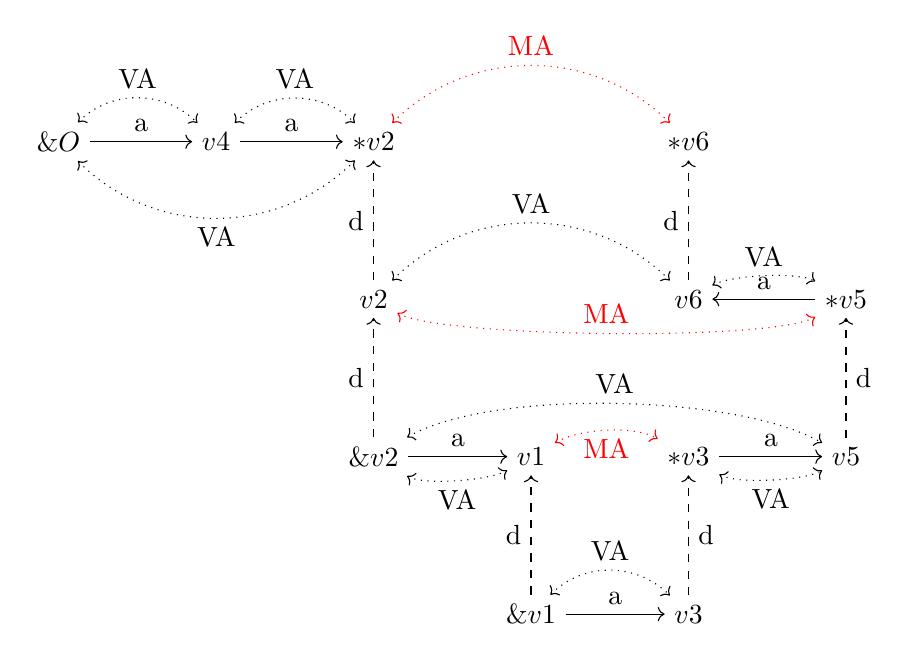
\begin{tikzpicture}[node distance=2cm] 
            \node[] (1) {$\&O$};
            \node[] (2) [right of=1] {$v4$}; 
            \node[] (3) [right of=2] {$*v2$};
            \node[] (4) [below of=3] {$v2$};
            \node[] (5) [below of=4] {$\&v2$};
            \node[] (6) [right of=5] {$v1$};
            \node[] (7) [below of=6] {$\&v1$};
            \node[] (8) [right of=7] {$v3$};
            \node[] (9) [above of=8] {$*v3$};
            \node[] (10) [right of=9] {$v5$};
            \node[] (11) [above of=10] {$*v5$};
            \node[] (12) [left of=11] {$v6$};
            \node[] (13) [above of=12] {$*v6$};
            \draw[->] (1) -- node[midway, above, sloped] {a} (2); 
            \draw[->] (2) -- node[midway, above, sloped] {a} (3); 
            \draw[dashed,->] (4) -- node[midway, left] {d} (3); 
            \draw[dashed,->] (5) -- node[midway, left] {d} (4); 
            \draw[->] (5) -- node[midway, above] {a} (6); 
            \draw[dashed,->] (7) -- node[midway, left] {d} (6); 
            \draw[->] (7) -- node[midway, above] {a} (8); 
            \draw[dashed,->] (8) -- node[midway, right] {d} (9); 
            \draw[->] (9) -- node[midway, above] {a} (10); 
            \draw[dashed,->] (10) -- node[midway, right] {d} (11); 
            \draw[->] (11) -- node[midway, above] {a} (12); 
            \draw[dashed,->] (12) -- node[midway, left] {d} (13); 
            
            \draw[dotted,<->] (1) to [out=45, in=135, looseness=1] node[midway, above] {VA} (2); 
            \draw[dotted,<->] (2) to [out=45, in=135, looseness=1] node[midway, above] {VA} (3); 
            \draw[dotted,<->] (1) to [out=-45, in=-135, looseness=1] node[midway, below] {VA} (3);
            \draw[dotted,<->,red] (3) to [out=45, in=135, looseness=1] node[midway, above,red] {MA} (13); 
            \draw[dotted,<->] (4) to [out=45, in=135, looseness=1] node[midway, above] {VA} (12); 
            \draw[dotted,<->,red] (4) to [out=-30, in=-150, looseness=0.3] node[midway, above,red] {MA} (11); 
            \draw[dotted,<->] (5) to [out=30, in=150, looseness=0.6] node[midway, above] {VA} (10); 
            \draw[dotted,<->] (5) to [out=-30, in=-150, looseness=0.5] node[midway, below] {VA} (6); 
            \draw[dotted,<->,red] (6) to [out=30, in=150, looseness=0.7] node[midway, below,red] {MA} (9); 
            \draw[dotted,<->] (7) to [out=45, in=135, looseness=1] node[midway, above] {VA} (8); 
            \draw[dotted,<->] (9) to [out=-30, in=-150, looseness=0.5] node[midway, below] {VA} (10);
            \draw[dotted,<->] (12) to [out=30, in=150, looseness=0.5] node[midway, above] {VA} (11); 
        \end{tikzpicture} 
    \end{subfigure}
    \caption{Анализ псевдонимов. Программа и её граф выражений}
    \label{fig:andersen_pag}
\end{figure}


Кроме задачи поиска всех пар псевдонимов можно выделить такие задачи, как проверка того, что два выражения являются псевдонимами, и поиск всех псевдонимов для выбранных выражений. Их можно переформулировать как задачу поиска путей с контекстно-свободными ограничениями с заданным множеством исходных вершин над тем же графом. Это позволит ускорить анализ, отказавшись от обработки неинтересующих вершин.

\subsection{Points-to анализ, учитывающий поля}
Ещё один вид анализа, который может быть сформулирован как задача поиска путей с контекстно-свободными ограничениями --- Points-to анализ, учитывающий поля, применяемый для анализа Java-программ. Он заключается в определении, на какие объекты кучи могли указывать переменные в процессе работы программы.

По исходной программе строится граф, вершины которого соответствуют объектам на куче и переменным программы, а рёбра добавляются на основании присваиваний по следующим правилам:

\begin{table}[H]
    \centering
    \begin{tabular}{ll}
        Выражение & Ребро в графе \\
        x = new Obj(); & $x \xrightarrow{alloc} h$ \\
        x = y; & $x \xrightarrow{assign} y$ \\
        x = y.f; & $x \xrightarrow{load_f} y$ \\
        x.f = y; & $x \xrightarrow{store_f} y$ \\
    \end{tabular}
\end{table}

Если достроить полученный граф обратными рёбрами: для каждого ребра $x \xrightarrow{label} y$ добавляется $x \xleftarrow{\overline{label}} y$, то такое представление программы позволяет сформулировать задачу анализа указателей как задачу поиска путей с контекстно-свободными ограничениями, задаваемую контекстно-свободной грамматикой:

\begin{table}[h]
    \centering
    \begin{tabular}{ll}
        $PointsTo\ \to\ (assign\ |\ load_f\ Alias\ store_f)^*$ $alloc$ & \\
        $Alias$ $\to$ $PointsTo$ \ $FlowsTo$ & $\forall$ f $\in$ $Fields$ \\
        $FlowsTo\ \to\ \overline{alloc}\ (\overline{assign}\ |\ \overline{store_f}\ Alias\ \overline{load_f})^*$ & \\
    \end{tabular}
\end{table}

На самом деле, это не КС-грамматика, а шаблон грамматики. Каждая программа обладает уникальным набором полей, поэтому грамматика, с помощью которой будет производиться анализ, будет получена из данного шаблона и графа, построенного по конкретной программе. Так, на рис.~\ref{fig:java_pag} представлен пример программы с тремя различными полями, построенный по ней граф выражений, дополненный рёбрами, которые показывают контекстно-свободную достижимость, задаваемую грамматикой.

\begin{figure}
    \begin{subfigure}{.3\textwidth}
        Программа \\ \\
        $v1 = new\ Obj();\ //\ h1$ \\
        $v2 = new\ Obj();\ //\ h2$ \\
        $v4 = new\ Obj();\ //\ h3$ \\
        $v6 = new\ Obj();\ //\ h4$ \\
        $v5 = v4;$ \\
        $v5 = v6;$ \\
        $v1.h = v1;$ \\
        $v2.g = v1;$ \\
        $v4.f = v2;$ \\
        $v7 = v5.f;$ \\
        $v9 = v6.f;$ \\
        $v3 = v2.g;$ \\
        $v8 = v7.g;$ \\
        $v10 = v9.g;$ \\
        $v10 = v10.h;$ \\
    \end{subfigure}
    \begin{subfigure}{.65\textwidth}
        \scalebox{0.8}{
        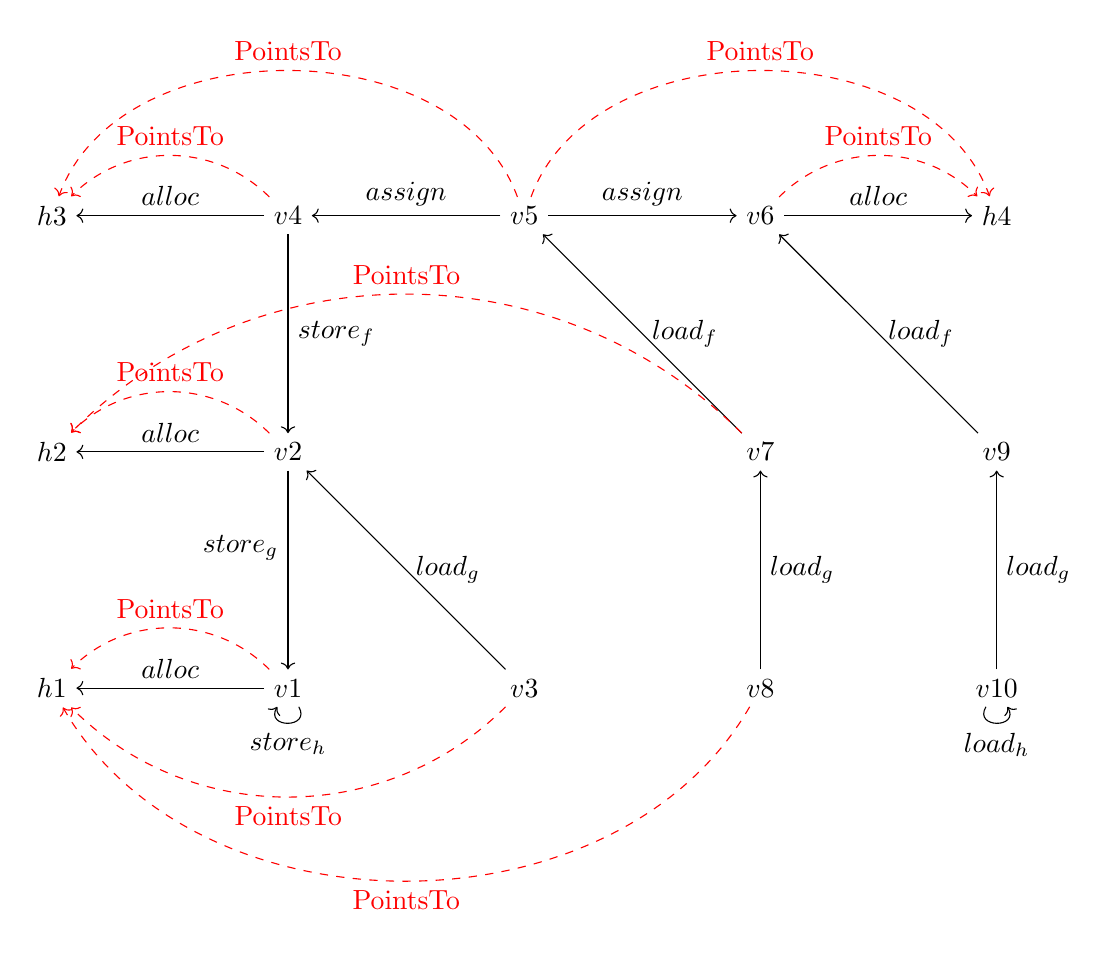
\begin{tikzpicture}[node distance=3cm] 
            \node[] (1) {$v5$};
            \node[] (2) [right of=1] {$v6$}; 
            \node[] (3) [left of=1] {$v4$};
            \node[] (4) [left of=3] {$h3$};
            \node[] (5) [right of=2] {$h4$};
            \node[] (6) [below of=3] {$v2$};
            \node[] (7) [left of=6] {$h2$};
            \node[] (8) [below of=2] {$v7$};
            \node[] (9) [below of=5] {$v9$};
            \node[] (10) [below of=6] {$v1$};
            \node[] (11) [left of=10] {$h1$};
            \node[] (12) [right of=10] {$v3$};
            \node[] (13) [below of=8] {$v8$};
            \node[] (14) [below of=9] {$v10$};
            \draw[->] (2) -- node[midway, above, sloped] {$alloc$} (5); 
            \draw[->] (3) -- node[midway, above, sloped] {$alloc$} (4); 
            \draw[->] (6) -- node[midway, above, sloped] {$alloc$} (7); 
            \draw[->] (10) -- node[midway, above, sloped] {$alloc$} (11); 
            \draw[->] (1) -- node[midway, above, sloped] {$assign$} (2); 
            \draw[->] (1) -- node[midway, above, sloped] {$assign$} (3);
            \draw[->] (14) to [out=-120, in=-60, looseness=3] node[midway, below] {$load_h$} (14); 
            \draw[->] (14) -- node[midway, right] {$load_g$} (9);
            \draw[->] (13) -- node[midway, right] {$load_g$} (8);
            \draw[->] (12) -- node[midway, right] {$load_g$} (6);
            \draw[->] (8) -- node[midway, right] {$load_f$} (1);
            \draw[->] (9) -- node[midway, right] {$load_f$} (2);
            \draw[->] (3) -- node[midway, right] {$store_f$} (6);
            \draw[->] (6) -- node[midway, above left] {$store_g$} (10);
            \draw[->] (10) to [out=-60, in=-120, looseness=3] node[midway, below] {$store_h$} (10); 
            
            \draw[dashed,->,red] (3) to [out=135, in=45, looseness=1] node[midway, above] {PointsTo} (4);
            \draw[dashed,->,red] (1) to [out=110, in=70, looseness=1] node[midway, above] {PointsTo} (4);
            \draw[dashed,->,red] (2) to [out=45, in=135, looseness=1] node[midway, above] {PointsTo} (5);
            \draw[dashed,->,red] (1) to [out=70, in=110, looseness=1] node[midway, above] {PointsTo} (5);
            \draw[dashed,->,red] (6) to [out=135, in=45, looseness=1] node[midway, above] {PointsTo} (7);
            \draw[dashed,->,red] (8) to [out=135, in=45, looseness=1] node[midway, above] {PointsTo} (7);
            \draw[dashed,->,red] (10) to [out=135, in=45, looseness=1] node[midway, above] {PointsTo} (11);
            \draw[dashed,->,red] (12) to [out=-135, in=-45, looseness=1] node[midway, below] {PointsTo} (11);
            \draw[dashed,->,red] (13) to [out=-120, in=-60, looseness=1] node[midway, below] {PointsTo} (11);
        \end{tikzpicture} 
    }
    \end{subfigure}
    \caption{Points-to анализ, учитывающий поля. Программа и её граф выражений}
    \label{fig:java_pag}
\end{figure}


\subsection{Алгоритмы КС-достижимости, основанные на операциях линейной алгебры}

Далее будут рассмотрены алгоритмы, решающие задачу контекстно-свободной достижимости, основанные на операциях линейной алгебры: матричном умножении и произведении Кронекера.

\subsubsection{Матричный алгоритм}

\begin{algorithm}
\small
\caption{Матричный алгоритм Рустама Азимова}
\label{alg:ap_matrix}
\begin{algorithmic}[1]
\Function{MatrixCFPQ}{$\mathcal{G}=(V,E,l)$, $G=(\Sigma, N, P, S)$}
    \State{$n \gets |V|$}
    \State{$M \gets \{M^A \mid  A \in N, M^A[i,j] \gets \textit{false} \text{, for all $i,j$}\} $}
    \ForAll{$v \in V$} \Comment{Инициализация матриц}
        \ForAll{$A \to \varepsilon$}
            \State{$M^A[v,v] \gets true$}
        \EndFor
    \EndFor
    \ForAll{$(v, u) \in E$} 
        \State{$label \gets l((v, u))$}
        \ForAll{$A \rightarrow label \in P$}
            \State{$M^A[u,v] \gets true$}
        \EndFor
    \EndFor    
    \While{$\exists A: M^A$ is changing}
    \Comment{Вычисление замыкания}
        \ForAll{$A \rightarrow BC \in P$}
            \State{$M^A \gets M^A + M^B \cdot M^C$}
        \EndFor
    \EndWhile
\State \Return $M^S$
\EndFunction

\end{algorithmic}
\end{algorithm}


В статье~\cite{rustam_algorithm} был преложен алгоритм, основанный на умножении матриц. На вход алгоритму подаётся граф $\mathcal{G}=\langle V,E,l \rangle$ и контекстно-свободная грамматика $G=\langle \Sigma, N, P, S\rangle$ в ослабленной нормальной форме Хомского.

Для каждого нетерминала $A \in N$ создаётся матрица смежности $M^A$. Если $M^A[i,j] = true$, то в графе между вершинами с номерами $i$ и $j$ существует путь, конкатенация меток на рёбрах которого образует слово, выводимое из нетерминала $A$ в заданной грамматике. Инициализация матриц происходит с помощью $\varepsilon$-правил: для правил вида $A \to \varepsilon$ для всех вершин добавляется петля $M^A[i,i] = true$, и простых правил грамматики (правил вида $A \to a$): если в графе между вершинами $i$ и $j$ есть ребро с меткой $a$, то $M^A[i,j] = true$.

Затем происходит поиск транзитивного замыкания (строки 15--19 алгоритма~\ref{alg:ap_matrix}), для правил вида $A \to BC$ матрица смежности нетерминала $A$ обновляется следующим образом: $M^A = M^A + M^B \cdot M^C$. Алгоритм использует булевы матрицы, поэтому в качестве сложения её элементов используется дизъюнкция, а в качестве умножения --- конъюнкция.

Результатом работы алгоритма является матрица смежности для стартового нетерминала --- $M^S$. Эта матрица будет содержать в себе информацию о всех парах вершин, соединённых путями, метки на рёбрах которых образуют слово из языка грамматики.


\subsubsection{Тензорный алгоритм}

Ещё один алгоритм КС-достижимости, основанный на операциях линейной алгебры --- алгоритм, основанный на произведении Кронекера~\cite{tensor_algorithm}. Алгоритм (листинг~\ref{alg:ap_tensor}) принимает граф $\mathcal{G}$ и рекурсивный автомат $R$. Его идея заключается в использовании модификации алгоритма пересечения конечных автоматов~\cite{automata_theory} для пересечения рекурсивного автомата и графа. Для этого граф $\mathcal{G}$ рассматривается как автомат: вершины считаются состояниями, а дуги --- переходами.

Входной граф и рекурсивный автомат представляются в виде композиции булевых матриц смежности для всех меток на рёбрах графа и переходах автомата. Пересечение выполняется с использованием произведения Кронекера, а множество рекурсивных вызовов учитывается с помощью транзитивного замыкания.

После инициализации матриц смежности проверяется наличие состояний в автомате $R$, которые одновременно являются стартовыми и конечными, и при наличии таковых для каждой вершины графа добавляется петля с соответствующей меткой.

Основной цикл алгоритма выполняется, пока набор матриц смежности для графа меняется. Первым шагом цикла происходит вычисление произведения Кронекера, тем самым создаётся матрица смежности нового автомата. Далее результат транзитивно замыкается для получения информации о достижимости состояний в полученном автомате. И последним шагом происходит обновление матрицы смежности графа.

\begin{algorithm}[]
    \small
    \begin{algorithmic}[1]
    \caption{Алгоритм, основанный на произведении Кронекера}
    \label{alg:ap_tensor}
    \Function{contextFreePathQuerying}{$\mathcal{G}$, $R$}
        % Input data preparation
        \State{$M_1 \gets$ набор матриц смежности для $R$} \Comment{Инициализация матриц}
        \State{$M_2 \gets$ набор матриц смежности для $\mathcal{G}$}
        \State{$n \gets$ dim$(M_1) \times $dim$(M_2)$}
        
        % Eps-transition handling for graph
        \For{$s \in 0..dim(\mathcal{M}_1)-1$}
            \For{$S \in \textit{getNonterminals}(R,s,s)$}
                \For{$i \in 0..dim(\mathcal{M}_2)-1$}
                    \State{$M_2^S[i,i] \gets \{1\}$}
                \EndFor
            \EndFor
        \EndFor
        \While{$M_2$ is changing} \Comment{Тело алгоритма}
            \State{$M_3 \gets M_1 \otimes M_2$} \Comment{Произведение Кронекера}
            \State{$C_3 \gets \textit{transitiveClosure}(M_3)$}
            \For{$i \in 0..n-1, j \in 0..n-1$}
                \If{$C_3[i,j]$}
                    \State{$s, f \gets \textit{getStates}(C_3,i,j)$}
                    \State{$x, y \gets \textit{getCoordinates}(C_3,i,j)$}
                    \For{$Nonterm \in \textit{getNonterminals}(R,s,f)$}
                        \State{$M_2^{Nonterm}[x,y] \gets \{1\}$}
                    \EndFor
                \EndIf
            \EndFor
        \EndWhile
    \State \Return $M_2$
    \EndFunction
    
    \Function{getStates}{$M_1, i, j$} \Comment{Получение номеров состояний автомата по номерам ячеек в матрице}
        \State{$r \gets dim(M_1)$}
        \State \Return{$\left\lfloor{i / r}\right\rfloor, \left\lfloor{j / r}\right\rfloor$}
    \EndFunction
    \Function{getCoordinates}{$M_2, i, j$} \Comment{Получение номеров вершин графа по индексам ячеек в матрице}
        \State{$n \gets dim(M_2)$}
        \State \Return{$i \bmod n, j \bmod n$}
    \EndFunction
    \end{algorithmic}
\end{algorithm}

\subsubsection{Инкрементальная версия тензорного алгоритма}

В работе~\cite{incremental_tensor_algorithm} предложена следующая оптимизация тензорного алгоритма. Чтобы вычислять произведение Кронекера инкрементально, можно воспользоваться левой дистрибутивностью данной операции. Пусть $A_2$ --- матрица, содержащая элементы, добавленные на последней итерации, $B_2$ --- матрица, содержащая элементы, добавленные ранее. Тогда в строке~13 алгоритма~\ref{alg:ap_tensor} по левой дистрибутивности $M_1 \otimes M_2 = M_1 \otimes (A_2 + B_2) = M_1 \otimes A_2 + M_1 \otimes B_2$. Однако $M_1 \otimes B_2$ уже был посчитан на предыдущей итерации, и его транзитивное замыкание хранится в $M_3$. Таким образом, остаётся обновить некоторые элементы $M_3$, вычислив $M_1 \otimes A_2$.

\subsection{Исследуемые реализации}
Ниже перечислены различные реализации, которые могут выполнять описанные виды статического анализа, сформулированные как задача КС-достижимости.

\begin{itemize}
    \item CFPQ\_PyAlgo\footnote{Репозиторий CFPQ\_PyAlgo: \url{https://github.com/FormalLanguageConstrainedPathQuerying/CFPQ_PyAlgo}, дата посещения 10.05.2023} --- платформа для разработки и тестирования алгоритмов запросов к графам с контекстно-свободными ограничениями, основанных на операциях линейной алгебры, содержащая реализации для: % CFPQ\_PyAlgo содержит реализации для:
    \begin{itemize}
        \item CPU: для выполнения операций с разреженными матрицами используется pygraphblas\footnote{Репозиторий pygraphblas: \url{https://github.com/Graphegon/pygraphblas}, дата посещения 22.05.2023} --- python-обёртка над библиотекой SuiteSparse\footnote{Репозиторий SuiteSparse: \url{https://github.com/DrTimothyAldenDavis/GraphBLAS}, дата посещения 22.05.2023};
        \item GPU: для выполнения операций с разреженными булевыми матрицами используется библиотека cuBool\footnote{Репозиторий cuBool: \url{https://github.com/SparseLinearAlgebra/cuBool}, дата посещения 22.05.2023}.
    \end{itemize}
    \item GLL4Graph\footnote{Репозиторий GLL4Graph: \url{https://github.com/FormalLanguageConstrainedPathQuerying/GLL4Graph}, дата посещения 22.05.2023} --- реализация алгоритма КС-достижимости, основанная на алгоритме синтаксического анализа GLL, написанная на Java. Поддерживает хранение графа в оперативной памяти и в графовой базе данных Neo4j.
    \item Graspan\footnote{Репозиторий Graspan-C: \url{https://github.com/Graspan/Graspan-C} Дата посещения 10.05.2023} --- высокопроизводительная система межпроцедурного статического анализа.
    \item Gigascale\footnote{Репозиторий Gigascale: \url{https://bitbucket.org/jensdietrich/gigascale-pointsto-oopsla2015/src/master/}, дата посещения 22.05.2023} --- высокопроизводительный инструмент для учитывающего поля Points-to анализа Java-программ. 
\end{itemize}

\section{Адаптация тензорного алгоритма для Points-to анализа, учитывающего поля}

% Расписать, почему матричный алгоритм плохо подходит
%Алгоритм, основанный на умножении матриц, требует создания булевой матрицы смежности для каждого нетерминала грамматики, поэтому для его практического применения необходимо, чтобы число нетерминалов грамматики в ослабленной нормальной форме Хомского было не очень велико.
Для практического применения алгоритма, основанного на умножении матриц, желательно, чтобы число нетерминалов грамматики в ослабленной нормальной форме Хомского было не очень велико, поскольку для каждого из них требуется создать булеву матрицу смежности. %енто перефразированное предложение
Например, в грамматике для анализа псевдонимов, переведённой в ослабленную нормальную форму Хомского, 12 нетерминалов. Однако число продукций в грамматике для Points-to анализа, учитывающего поля, зависит от числа полей анализируемой программы и может достигать нескольких тысяч. Это делает матричный алгоритм плохо применимым.

% Расписать, почему тензорный алгоритм алгоритм плохо подходит
В алгоритме, основанном на произведении Кронекера, для пересечения рекурсивного автомата и ориентированного графа они представляются как композиция булевых матриц смежности для всех различных меток на рёбрах. На рис.~\ref{fig:java_rsm} представлен рекурсивный автомат для Points-to анализа, учитывающего поля. Можно заметить, что все метки на рёбрах, кроме Alias, встречаются по одному разу.
%Поэтому для всех этих меток будет создана булева матрица смежности, содержащая единственный элемент, для всех этих матриц необходимо считать произведение Кронекера с соответствующей матрицей смежности графа, а затем складывать полученный результат.
Поэтому для всех этих меток будет создана булева матрица смежности, содержащая единственный элемент, и для каждой из них необходимо считать произведение Кронекера с соответствующей матрицей смежности графа, а затем складывать полученный результат.%хз, насколько удачно убран повтор "матриц"

\begin{figure}[h]
  \begin{tabular}{|c|c|c|}
    \hline
    PointsTo & FlowsTo & Alias \\
      % Программа & Граф выражений \\
      
      \begin{minipage}{.37\textwidth}
      \scalebox{0.6}{
      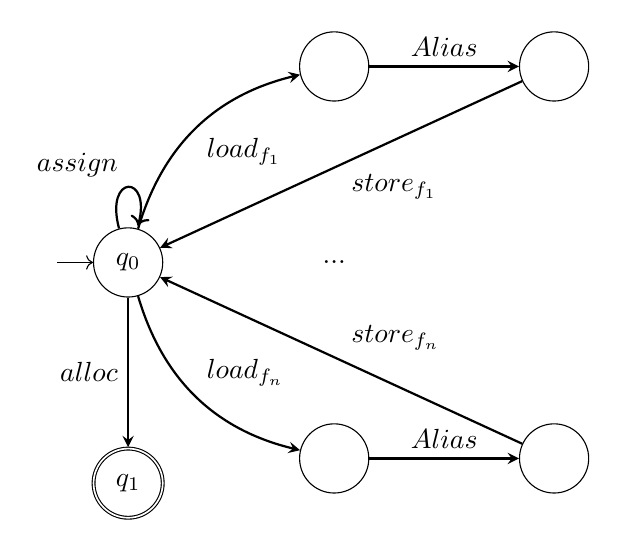
\begin{tikzpicture}[node distance=1.9cm, auto] 
          \node (q0) [state, initial, initial text = {}] {$q_0$};
          \node (q1) [state, accepting, below = of q0] {$q_1$};
          
          \node (q4) [right = of q0] {$...$};
          
          \node (q2) [state, above = of q4] {};
          \node (q3) [state, right = of q2] {};
          
          \node (q5) [state, below = of q4] {};
          \node (q6) [state, right = of q5] {};
          
          \path [-stealth, thick]
              (q0) edge [loop above]  node[above left] {$assign$}()
              (q0) edge node[left] {$alloc$} (q1)
              
              (q0) edge[bend left] node[below right] {$load_{f_1}$} (q2)
              (q2) edge node[above] {$Alias$} (q3)
              (q3) edge node[below right] {$store_{f_1}$} (q0)
              
              (q0) edge[bend right] node[above right] {$load_{f_n}$} (q5)
              (q5) edge node[above] {$Alias$} (q6)
              (q6) edge node[above right] {$store_{f_n}$} (q0)
              ;
      \end{tikzpicture}
      }
      \end{minipage}
  
      &
  \begin{minipage}{.38\textwidth}
  \scalebox{0.6}{
      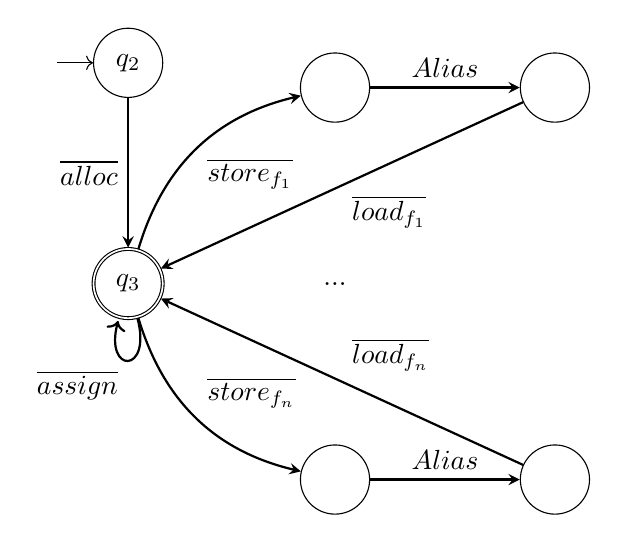
\begin{tikzpicture}[node distance=1.9cm] 
          \node (q0) [state, initial, initial text = {}] {$q_2$};
          \node (q1) [state, accepting, below = of q0] {$q_3$};
          
          \node (q4) [right = of q1] {$...$};
          
          \node (q2) [state, above = of q4] {};
          \node (q3) [state, right = of q2] {};
          
          \node (q5) [state, below = of q4] {};
          \node (q6) [state, right = of q5] {};
          
          \path [-stealth, thick]
              (q0) edge node[left] {$\overline{alloc}$} (q1)
              (q1) edge [loop below] node[below left] {$\overline{assign}$}()
              
              (q1) edge[bend left] node[below right] {$\overline{store_{f_1}}$} (q2)
              (q2) edge node[above] {$Alias$} (q3)
              (q3) edge node[below right] {$\overline{load_{f_1}}$} (q1)
              
              (q1) edge[bend right] node[above right] {$\overline{store_{f_n}}$} (q5)
              (q5) edge node[above] {$Alias$} (q6)
              (q6) edge node[above right] {$\overline{load_{f_n}}$} (q1);
      \end{tikzpicture} 
      }
      \end{minipage}
      &
  \begin{minipage}{.17\textwidth}
  \scalebox{0.7}{
      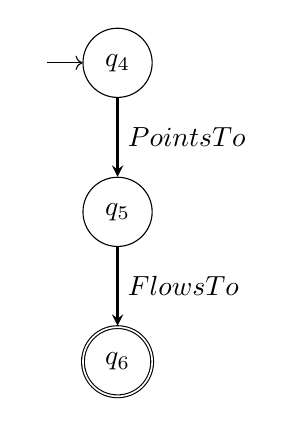
\begin{tikzpicture}[node distance=1.0cm] 
          \node (q0) [state, initial, initial text = {}] {$q_4$};
          \node (q1) [state, below = of q0] {$q_5$};
          \node (q2) [state, accepting, below = of q1] {$q_6$};
          \path [-stealth, thick]
              (q0) edge node[right] {$PointsTo$} (q1)
              (q1) edge node[right] {$FlowsTo$} (q2)
              ;
      \end{tikzpicture} 
      }
      \end{minipage}
      \\
      & & \\
      \hline
  
  \end{tabular}
  \caption{Рекурсивный автомат для Points-to анализа, учитывающего поля}
  \label{fig:java_rsm}
\end{figure}

% Расписать, как улучшили тензорный алгоритм
С целью уменьшения числа операций был рассмотрен другой способ представления графа и рекурсивного автомата в виде матриц. Стоит отметить, что в этом рекурсивном автомате переход между любыми двумя состояниями происходит только по одной метке. Это позволяет представить его одной матрицей смежности, элементы которой --- целые числа. Старшие два бита этого числа содержат номер нетерминала, остальные --- номер терминала (рис.~\ref{fig:java_graph_representation}).

\begin{figure}[h!]
  \centering
  \begin{tikzpicture}
    [%%%%%%%%%%%%%%%%%%%%%%%%%%%%%%
        box/.style={rectangle,draw=black, ultra thick, minimum size=1cm},
    ]%%%%%%%%%%%%%%%%%%%%%%%%%%%%%%
    \foreach \x in {0,1,2,3,4,5,6,7,8}
        \node[box] at (\x,0){};
    \draw[decorate,decoration={brace, amplitude=0.2cm,mirror},thick] (-.5,-.7) -- node[below]{Нетерминал} (1.49,-.7);
    \draw[decorate,decoration={brace, amplitude=0.2cm, mirror},thick] (1.51,-.7) -- node[below]{Терминал} (8.5,-.7);
  \end{tikzpicture}
  \caption{Представление элементов матрицы смежности графа и рекурсивного автомата}
  \label{fig:java_graph_representation}
\end{figure}

В результате данного анализа между двумя вершинами в графе может быть добавлено ребро только с одним из трёх нетерминалов:
\begin{itemize}
    \item PointsTo --- между вершиной, соответствующей переменной, и вершиной, соответствующей объекту кучи;
    \item FlowsTo --- между вершиной, соответствующей объекту кучи, и вершиной, соответствующей переменной;
    \item Alias --- между двумя вершинами, соответствующими переменным.
\end{itemize}

Если во входном графе между двумя вершинами будет не больше одного ребра, то для графа можно будет использовать такое же представление, как и для рекурсивного автомата. Однако способ построения графа по программе этого не гарантирует. Можно преобразовать входной граф так, чтобы он соответствовал этому требованию и по результату анализа этого графа можно было легко получить результаты для исходного. Если между парой вершин есть несколько рёбер, то можно разбить одно из них на два, добавив вершину, задающую новую переменную, как показано на рис.~\ref{fig:java_graph_transform}. Такое преобразование графа не влияет на результат анализа для исходных вершин.

\begin{figure}
  \begin{tabular}{ccc}
    Исходные рёбра & Новая переменная & Результат \\
   
    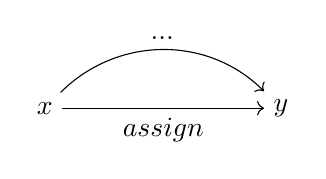
\begin{tikzpicture}[node distance=3.0cm] 
          \node[] (1) {$x$};
          \node[] (2) [right of=1] {$y$};
          
          \draw[->] (1) to [out=45, in=135, looseness=1] node[midway, above] {$...$} (2);
          \draw[->] (1) to node[midway, below, sloped] {$assign$} (2); 
    \end{tikzpicture} 
    &
    z = y; x = z;
    & 
    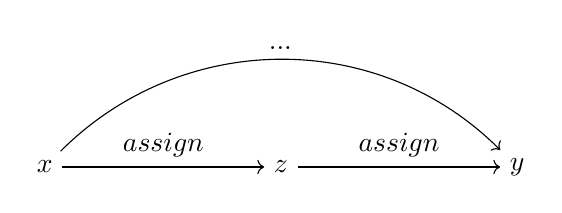
\begin{tikzpicture}[node distance=3.0cm] 
          \node[] (1) {$x$};
          \node[] (2) [right of=1] {$z$};
          \node[] (3) [right of=2] {$y$};
          
          \draw[->] (1) -- node[midway, above, sloped] {$assign$} (2); 
          \draw[->] (2) -- node[midway, above, sloped] {$assign$} (3); 
          \draw[->] (1) to [out=45, in=135, looseness=1] node[midway, above] {$...$} (3);
    \end{tikzpicture} 
    \\
    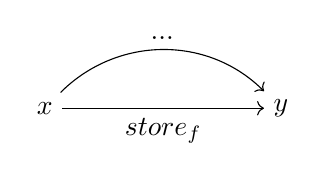
\begin{tikzpicture}[node distance=3.0cm] 
          \node[] (1) {$x$};
          \node[] (2) [right of=1] {$y$};
          
          \draw[->] (1) to [out=45, in=135, looseness=1] node[midway, above] {$...$} (2);
          \draw[->] (1) to node[midway, below, sloped] {$store_f$} (2); 
    \end{tikzpicture} 
    &
    z = y; x.f = z;
    & 
    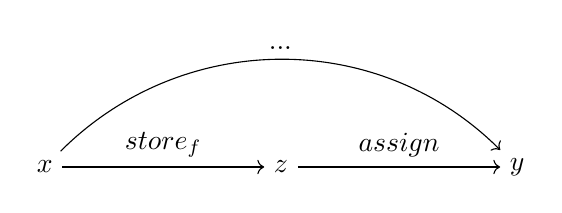
\begin{tikzpicture}[node distance=3.0cm] 
          \node[] (1) {$x$};
          \node[] (2) [right of=1] {$z$};
          \node[] (3) [right of=2] {$y$};
          
          \draw[->] (1) -- node[midway, above, sloped] {$store_f$} (2); 
          \draw[->] (2) -- node[midway, above, sloped] {$assign$} (3); 
          \draw[->] (1) to [out=45, in=135, looseness=1] node[midway, above] {$...$} (3);
    \end{tikzpicture} 
    \\
    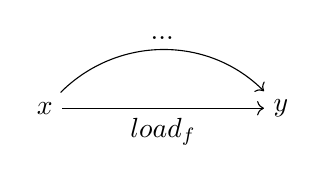
\begin{tikzpicture}[node distance=3.0cm] 
          \node[] (1) {$x$};
          \node[] (2) [right of=1] {$y$};
          
          \draw[->] (1) to [out=45, in=135, looseness=1] node[midway, above] {$...$} (2);
          \draw[->] (1) to node[midway, below, sloped] {$load_f$} (2); 
    \end{tikzpicture} 
    &
    z = y.f; x = z;
    & 
    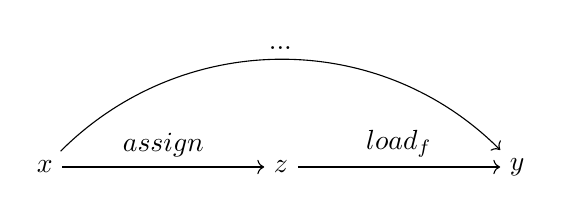
\begin{tikzpicture}[node distance=3.0cm] 
          \node[] (1) {$x$};
          \node[] (2) [right of=1] {$z$};
          \node[] (3) [right of=2] {$y$};
          
          \draw[->] (1) -- node[midway, above, sloped] {$assign$} (2); 
          \draw[->] (2) -- node[midway, above, sloped] {$load_f$} (3); 
          \draw[->] (1) to [out=45, in=135, looseness=1] node[midway, above] {$...$} (3);
    \end{tikzpicture} 
    \end{tabular}
    \caption{Адаптация графа}
  \label{fig:java_graph_transform}
\end{figure}


Поскольку для пересечения автомата и графа применяется произведение Кронекера, необходимо задать бинарную операцию умножения для элементов матриц смежности описанного формата. Если ребро в графе и ребро в автомате содержат одинаковый нетерминал или одинаковый терминал, то соответствующая ячейка в результате произведения Кронекера будет $true$, иначе --- $false$. Эту операцию можно задать так: $times(x, y) = (x_{nonterm} = y_{nonterm} \neq 0 \ or\ x_{term} = y_{term} \neq 0)$. Данное представление графа и рекурсивного автомата в виде матриц с применением такой операции позволяет на каждой итерации алгоритма вычислять произведение Кронекера всего один раз.

\subsection{Применение модификации для анализа псевдонимов}

На рис.~\ref{fig:ma_rsm} представлен рекурсивный автомат для анализа псевдонимов. В нём переход между любыми двумя состояниями происходит только по одной метке, поэтому для него можно использовать описанное выше представление. Однако в результате анализа между двумя вершинами могут быть добавлены как ребро $MA$, так и ребро $VA$. Поэтому необходимо иметь возможность хранить два нетерминала на ребре.

\begin{figure}[h]
  \begin{tabular}{|c|c|}
    \hline
    MA & VA \\
      % Программа & Граф выражений \\
      
      \begin{minipage}{.53\textwidth}
      \scalebox{0.7}{
      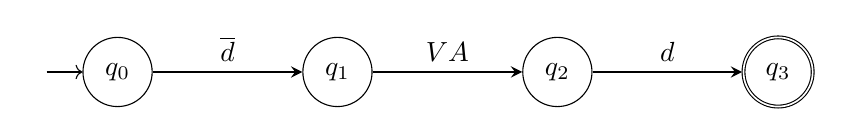
\begin{tikzpicture}[node distance=1.9cm, auto] 
          \node (q0) [state, initial, initial text = {}] {$q_0$};
          \node (q1) [state, right = of q0] {$q_1$};
          \node (q2) [state, right = of q1] {$q_2$};
          \node (q3) [state, accepting, right = of q2] {$q_3$};
          
          \path [-stealth, thick]
              (q0) edge node[above] {$\overline{d}$} (q1)
              (q1) edge node[above] {$VA$} (q2)
              (q2) edge node[above] {$d$} (q3)
              ;
      \end{tikzpicture}
      }
      \end{minipage}
  
      &
  \begin{minipage}{.43\textwidth}
  \scalebox{0.7}{
      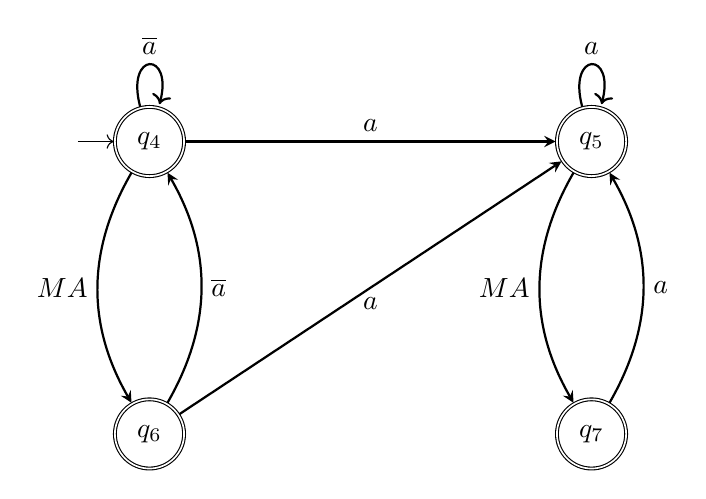
\begin{tikzpicture}[node distance=2.8cm, auto] 
          \node (q0) [state, accepting, initial, initial text = {}] {$q_4$};
          \node (q1) [state, accepting, right=4.7cm of q0] {$q_5$};
          \node (q2) [state, accepting, below = of q0] {$q_6$};
          \node (q3) [state, accepting, below = of q1] {$q_7$};
          
          \path [-stealth, thick]
              (q0) edge node[above] {$a$} (q1)
              (q0) edge [loop above] node[above] {$\overline{a}$}()
              (q0) edge[bend right] node[left] {$MA$} (q2)

              (q1) edge[loop above] node[above] {$a$}()
              (q1) edge[bend right] node[left] {$MA$} (q3)

              (q2) edge[bend right] node[right] {$\overline{a}$} (q0)
              (q2) edge node[below] {$a$} (q1)
              
              (q3) edge[bend right] node[right] {$a$} (q1)
              ;
      \end{tikzpicture} 
      }
      \end{minipage}
      \\
      & \\
      \hline
  
  \end{tabular}
  \caption{Рекурсивный автомат для анализа псевдонимов}
  \label{fig:ma_rsm}
\end{figure}


Чтобы хранить несколько нетерминалов на ребре, старшие биты числа, содержащего информацию о ребре, будут содержать не номер нетерминала, а маску для всех возможных нетерминалов. Тогда можно задать операцию умножения элементов для произведения Кронекера так: $times(x, y) = (x_{nonterm} \& y_{nonterm} \neq 0 \ or\ x_{term} = y_{term} \neq 0)$.


Стоит отметить, что такое представление также подойдёт для Points-to анализа, учитывающего поля, но оно потребует отдать под нетерминалы на один бит больше. Это может негативно сказаться на потреблении памяти: если под хранение терминала в числе не будет хватать памяти, придётся брать более длинный целочисленный тип для хранения.


\subsection{Особенности реализации}

Данная модификация тензорного алгоритма и её инкрементальная версия были реализованы в библиотеке CFPQ\_PyAlgo\footnote{\url{https://github.com/FormalLanguageConstrainedPathQuerying/CFPQ_PyAlgo/tree/vkutuev/ot_tensor}, пользователь vkutuev. Дата посещения 22.05.2023}, в которой для работы с разреженными матрицами используется библиотека pygraphblas, являющаяся python-обёрткой над библиотекой SuiteSparse. 

При использовании предложенной операции умножения элементов матрицы после произведения Кронекера большинство элементов матрицы-результата будут $false$. Это приводит к двум проблемам: 
\begin{enumerate}
    \item вычисление транзитивного замыкания потребует больше времени, так как матрица содержит больше элементов;
    \item необходимо выделить больше памяти под хранение этой матрицы.
\end{enumerate}

Очистка матрицы от значений $false$ после транзитивного замыкания поможет решить первую проблему. Однако потребность выделить дополнительную память под незначащие элементы матрицы может привести к нехватке памяти. 

Для решения этой проблемы были внесены изменения в исходный код функции, вычисляющей произведение Кронекера, в библиотеке SuiteSparse\footnote{\url{https://github.com/vkutuev/GraphBLAS/tree/vkutuev/kron}, пользователь vkutuev. Дата посещения 22.05.2023}: перед выделением памяти под матрицу-результат производится вычисление количества значащих элементов в результате, и выделение памяти происходит только под это число элементов. Благодаря этому подходу удалось снизить пиковое потребление памяти. На рис.~\ref{fig:memory_profile_a} представлен профиль памяти работы алгоритма со стандартной реализацией произведения Кронекера из библиотеки SuiteSparse с последующей фильтрацией результата, пиковое потребление памяти --- 5,2 ГиБ. А на рис.~\ref{fig:memory_profile_b} --- профиль памяти работы алгоритма с доработанной реализацией, выделяющей память только под элементы результата, которые будут $true$, пиковое потребление памяти --- 2,3 ГиБ.

\begin{figure}[]
    \begin{subfigure}{\textwidth}
        \centering
        \includegraphics[width=\linewidth]{figures/mem_prof_base.pdf}
        \caption{Стандартная реализация}
        \label{fig:memory_profile_a}
    \end{subfigure}
    \begin{subfigure}{\textwidth}
        \centering
        \includegraphics[width=\linewidth]{figures/mem_prof_patched.pdf}
        \caption{Оптимизированная реализация}
        \label{fig:memory_profile_b}
    \end{subfigure}
    \caption{Профиль потребления памяти на одном графе с разными реализациями произведения Кронекера}
    \label{fig:memory_profile}
\end{figure}


\section{Оптимизация реализации матричного алгоритма}

В pygraphblas при умножении двух матриц необходимо передать методу умножения полукольцо, в котором происходит сложение и умножение элементов матрицы. В реализации алгоритмов поиска путей с контекстно-свободными ограничениями используются разреженные булевы матрицы, поэтому для умножения использовалось полукольцо BOOL.LOR\_LAND: домен --- булевы значения $\{true$, $false\}$, сложение --- LOR (дизъюнкция), умножение --- LAND (конъюнкция). Однако разреженность матриц меняет множество значений, которые может принимать элемент матрицы: $true$, $false$ и <<нет значения>>. При этом в реализации матричного алгоритма элементы матрицы никогда не принимают значения $false$. Изначально во всех матрицах нет значений, затем некоторые элементы матрицы в соответствии с простыми правилами грамматики инициализируются значением $true$. Затем в матрицу могут добавляться только значения $true$, если была найдена новая пара вершин, между которыми существует путь. Таким образом, полукольцо BOOL.LOR\_LAND является избыточным для реализации данного алгоритма. Для избавления от этой избыточности можно воспользоваться полукольцом с операциями ANY (выбирает любой из переданных аргументов) в качестве сложения и PAIR (возвращает 1 в полукольце, если оба операнда --- присутствующие в матрице элементы) в качестве умножения. В силу того, как заполняется матрица в данном алгоритме, использование полукольца BOOL.ANY\_PAIR при умножении матриц не изменит результат умножения, но операции ANY и PAIR проще и выполняются быстрее, чем LOR и LAND.

Данная оптимизация была применена в реализации матричного алгоритма в CFPQ\_PyAlgo\footnote{\url{https://github.com/FormalLanguageConstrainedPathQuerying/CFPQ_PyAlgo}, пользователь vkutuev. Дата посещения 22.05.2023}.
\section{Эксперименты}

\subsection{Тестовый стенд}

Для замеров времени работы алгоритмов использовался компьютер со следующими характеристиками:
\begin{itemize}
    \item CPU: Intel(R) Core(TM) i7-479, тактовая частота: 3.6 ГГц, 4 ядра, 4 потока;
    \item ОЗУ: 64 ГиБ;
    \item GPU: GeForce GTX 1070 GPU (8 ГиБ памяти DDR5).
\end{itemize}


Для проведения экспериментов использовалось следующее программное обеспечение:
\begin{itemize}
    \item операционная система: Ubuntu 20.04;
    \item Python: 3.8.10;
    \item Java: 15.0.2;
    \item GCC: 9.4.0.
\end{itemize}

\subsection{Тестовые данные}
Для проведения экспериментов были взяты графы из набора CFPQ\_Data, построенные по реальным программам. Описание графов для анализа псевдонимов и Points-to анализа, учитывающего поля, представлены в таблицах~\ref{tab:graphs_descr_ma} и~\ref{tab:graphs_descr_java}. 

\begin{table}[h!]
    \centering
    \resizebox{.7\textwidth}{!}{%
    \begin{tabular}{|l|r|r|r|}
    \hline
    Граф & $|V|$ & $|E|$ & Число пар  \\ 
     & & & достижимых вершин  \\ \hline
    wc & 332 & 269 & 156 \\ \hline
    bzip2 & 632 & 556 & 315 \\ \hline
    pr & 815 & 692 & 385 \\ \hline
    ls & 1 687 & 1 453 & 854 \\ \hline
    gzip & 2 687 & 2 293 & 1 458 \\ \hline
    apache & 1 721 418 & 1 510 411 & 92 806 768 \\ \hline
    init & 2 446 224 & 2 112 809 & 3 783 769 \\ \hline
    mm & 2 538 243 & 2 191 079 & 3 990 305 \\ \hline
    ipc & 3 401 022 & 2 931 498 & 5 249 389 \\ \hline
    lib & 3 401 355 & 2 931 880 & 5 276 303 \\ \hline
    block & 3 423 234 & 2 951 393 & 5 351 409 \\ \hline
    arch & 3 448 422 & 2 970 242 & 5 339 563 \\ \hline
    crypto & 3 464 970 & 2 988 387 & 5 428 237 \\ \hline
    security & 3 479 982 & 3 003 326 & 5 593 387 \\ \hline
    sound & 3 528 861 & 3 049 732 & 6 085 269 \\ \hline
    net & 4 039 470 & 3 500 141 & 8 833 403 \\ \hline
    fs & 4 177 416 & 3 609 373 & 9 646 475 \\ \hline
    drivers & 4 273 803 & 3 707 769 & 18 825 025 \\ \hline
    postgre & 5 203 419 & 4 678 543 & 90 661 446 \\ \hline
    kernel & 11 254 434 & 9 484 213 & 16 747 731 \\ \hline
    \end{tabular}%
    }
    \caption{Описание графов из тестового набора для анализа псевдонимов}
\label{tab:graphs_descr_ma}
\end{table}

\begin{table}[h!]
    \centering
    \resizebox{.7\textwidth}{!}{%
    \begin{tabular}{|l|r|r|r|}
    \hline
    Граф & $|V|$ & $|E|$ & Число пар  \\ 
     & & & достижимых вершин  \\ \hline
    sunflow & 15464 & 15957 & 16354 \\ \hline
    lusearch & 15774 & 14994 & 9242 \\ \hline
    luindex & 18532 & 17375 & 9677 \\ \hline
    avrora & 24690 & 25196 & 21532 \\ \hline
    eclipse & 41383 & 40200 & 21830 \\ \hline
    batik & 60175 & 63089 & 45968 \\ \hline
    fop & 86183 & 83016 & 76615 \\ \hline
    pmd & 54444 & 59329 & 60518 \\ \hline
    xalan & 58476 & 62758 & 52382 \\ \hline
    h2 & 44717 & 56683 & 92038 \\ \hline
    tomcat & 111327 & 110884 & 82424 \\ \hline
    \end{tabular}%
    }
    \caption{Описание графов из тестового набора для Points-to анализа, учитывающего поля}
\label{tab:graphs_descr_java}
\end{table}

\subsection{Замеры времени работы и потреблетния памяти}

Для проведения замеров производительности каждая реализация запускалась на каждом анализируемом графе по 30 раз. При замерах времени работы учитывалось только время обработки уже загруженных в память графа и грамматики.

Для замеров времени работы реализаций из CFPQ\_PyAlgo использовался пакет benchmark, входящий в репозиторий, позволяющий задать замеряемую реализацию, входные данные и количество измерений, которые необходимо провести. Для замеров памяти CPU-реализаций измерялся Resident Set Size (RSS) процесса, а для GPU-реализаций измерялось потребление видеопамяти профилятором\footnote{\url{https://github.com/EgorOrachyov/SpBench/blob/main/scripts/gpu_mem_prof.py}, дата посещения 22.05.2023}, основанным на nvidia-smi\footnote{\url{https://developer.nvidia.com/nvidia-system-management-interface}, дата посещения 22.05.2023}.

Для проведения замеров времени работы и потребляемой памяти реализации, основанной на алгоритме синтаксического анализа GLL, в реализацию были внесены изменения\footnote{\url{https://github.com/FormalLanguageConstrainedPathQuerying/GLL4Graph/tree/vkutuev/memory_usage}, пользователь vkutuev. Дата посещения 22.05.2023}, позволяющие проводить замеры времени работы и потребления памяти с произвольной контекстно-свободной грамматикой, с указанным хранилищем для графа, с заданным числом итераций для прогрева JVM и для замеров.

Graspan позволяет получить время обработки загруженного в память графа, однако не позволяет получить информацию о потребляемой памяти. Для получений объёма затраченной памяти измерялся RSS процесса.

Gigascale позволяет получить как время обработки загруженного графа, так и объём затраченной памяти.

\subsection{Оптимизация реализации матричного алгоритма}

Чтобы оценить влияние предложенной оптимизации, было измерено время работы с ней и без неё. Для сравнения реализаций были взяты графы apache и init, а также графы меньшего размера из CFPQ\_Data. Результаты замеров с использованием разных полуколец для перемножения матриц представлены в таблице~\ref{tab:any_pair_res}.


\begin{table}[h!]
    \centering
    \begin{tabular}{|l|r|r|r|}
    \hline
    Граф & LOR\_LAND (сек.) & ANY\_PAIR (сек.) & Ускорение \\ \hline
    wc & 0,006 & 0,006 & 1,00 \\ \hline
    bzip2 & 0,022 & 0,022 & 1,00 \\ \hline
    pr & 0,013 & 0,012 & 1,08 \\ \hline
    ls & 0,051 & 0,045 & 1,13 \\ \hline
    gzip & 0,038 & 0,030 & 1,26 \\ \hline
    apache & 683,58 & 536,70 & 1,27 \\ \hline
    init & 59,33 & 45,84 & 1,29 \\ \hline
    \end{tabular}%
\caption{Влияние оптимизации на время работы}
\label{tab:any_pair_res}
\end{table}

Полученные результаты показывают, что для графов небольшого размера данная оптимизация практически не влияет на время работы, однако с ростом графов возрастает и ускорение, которое она даёт.

\subsection{Сравнение алгоритмов КС-достижимости}

В ходе экспериментов сравнивались следующие реализации:
\begin{itemize}
    \item реализации матричного алгоритма из CFPQ\_PyAlgo для CPU (\textbf{MC}) и GPU (\textbf{MG});
    \item реализация тензорного алгоритма из CFPQ\_PyAlgo для CPU (\textbf{KC}) и GPU (\textbf{KG}), инкрементальная версия тензорного алгоритма (\textbf{DKC});
    \item реализация адаптированного для Points-to анализа, учитывающего поля, тензорного алгоритма (\textbf{OTKC}) и его инкрементальная версия (\textbf{OTDKC});
    \item реализация алгоритма, основанного на алгоритме синтаксического анализа \textbf{GLL} (запускалась вариация с хранением графа в оперативной памяти);
    \item \textbf{Graspan} (запускался только для анализа псевдонимов, так как эта реализация не поддерживает грамматики с большим количеством нетерминалов);
    \item \textbf{Gigascale} (запускался только для Points-to анализа, учитывающего поля, так как эта реализация заточена под конкретную грамматику).
\end{itemize}

На рис.~\ref{fig:ma_result} и \ref{fig:java_result} представлены результаты замеров времени работы и потребления памяти данных реализаций. Результаты некоторых запусков не отображаются, если время работы превышает 5 часов или запуск завершился с ошибкой из-за нехватки памяти. 
\begin{figure}[h!]
    \begin{subfigure}{\textwidth}
        \centering
        \includegraphics[width=\linewidth, height=8.1cm]{figures/ma_time.pdf}
        \caption{Время работы}
        \label{fig:ma_result_time}
    \end{subfigure}
    \begin{subfigure}{\textwidth}
        \centering
        \includegraphics[width=\linewidth, height=8.1cm]{figures/ma_mem.pdf}
        \caption{Потребление памяти}
        \label{fig:ma_result_mem}
    \end{subfigure}
    \caption{Результаты для анализа псевдонимов}
    \label{fig:ma_result}
\end{figure}

\begin{figure}[h!]
    \begin{subfigure}{\textwidth}
        \centering
        \includegraphics[width=\linewidth, height=8cm]{figures/java_time.pdf}
        \caption{Время работы}
        \label{fig:java_result_time}
    \end{subfigure}
    \begin{subfigure}{\textwidth}
        \centering
        \includegraphics[width=\linewidth, height=8cm]{figures/java_mem.pdf}
        \caption{Потребление памяти}
        \label{fig:java_result_mem}
    \end{subfigure}
    \caption{Результаты для Points-to анализа, учитывающего поля}
    \label{fig:java_result}
\end{figure}

На основе полученных в результате экспериментов данных можно сделать следующие выводы.

\begin{itemize}
    \item При анализе псевдонимов наилучшие результаты (как время работы, так и потребление памяти) показала реализация матричного алгоритма для GPU. Для CPU же наименьшее время работы продемонстрировал Graspan. Однако при наличии в ответе большого числа пар достижимых вершин он работает значительно медленнее реализаций матричного алгоритма.
    \item Наименьшие время работы и потребление памяти при Points-to анализе, учитывающем поля, показала реализация Gigascale, работающая значительно быстрее всех остальных реализаций, что вполне обоснованно, ведь данный инструмент был разработан именно для такого анализа.
    \item Предложенные в работе модификация тензорного алгоритма и её инкрементальная версия работают быстрее других реализаций алгоритма для CPU в обоих видах анализа. Также можно отметить, что на небольших графах для Points-to анализа, учитывающего поля, инкрементальная версия продемонстрировала наименьшее время работы среди всех алгоритмов, основанных на операциях линейной алгебры. Однако эта реализация, как и базовый тензорный алгоритм, обладает таким недостатком, как большое потребление памяти. Это связано с большим размером получаемой в результате произведения Кронекера матрицы, который зависит и от размеров графа, и от размеров грамматики, что привело к ошибке нехватки памяти на графах fop, pmd, xalan, h2 и tomcat.
\end{itemize}


\section*{Заключение}
В ходе работы были достигнуты следующие результаты.
\begin{itemize}
    \item Предложена модификация тензорного алгоритма для Points-to анализа, учитывающего поля, показавшая наилучшее время работы на небольших графах среди алгоритмов, основанных на операциях линейной алгебры. Однако эксперименты показали, что из-за большого потребления памяти алгоритм практически неприменим для данного вида анализа.
    \item Оптимизирована реализация матричного алгоритма из библиотеки CFPQ\_PyAlgo, эффективность оптимизации экспериментально проверена.
    \item Проведены замеры производительности реализаций алгоритмов КС-достижимости, которые показали, что алгоритмы, основанные на операциях линейной алгебры, достаточно эффективны для анализа псевдонимов, но из-за больших размеров грамматики малоэффективны для Points-to анализа, учитывающего поля.
\end{itemize}

Так как реализации алгоритма, основанного на произведении Кронекера, и его вариации плохо применимы для Points-to анализа, учитывающего поля, в силу очень большого объёма потребляемой памяти под пересечение графа и рекурсивного автомата, в дальнейшем можно рассмотреть следующие шаги по оптимизации матричного алгоритма для применения его к данному типу анализа.
\begin{itemize}
    \item Разработка инкрементальной версии матричного алгоритма, в которой полученные на предыдущих итерациях данные не будут пересчитываться в дальнейшем, что позволит сократить затрачиваемое на умножение матриц время.
    \item Специализация матричного алгоритма для данного анализа, не требующего перевода грамматики в ОНФХ и вычисления достижимости для нетерминала $FlowsTo$ непосредственно, что позволит значительно сократить количество перемножений матриц.
\end{itemize}


\setmonofont[Mapping=tex-text]{CMU Typewriter Text}
\bibliographystyle{ugost2008ls}
\bibliography{report.bib}
\end{document}

